\section{Inequação do 2° grau}

\begin{definition}
    Uma \textdef{inequação do segundo grau} é uma relação de uma das formas
    a seguir:
    \begin{align*}
        ax^2 + bx + c &< 0;   \\
        ax^2 + bx + c &> 0;   \\
        ax^2 + bx + c &\le 0; \\
        ax^2 + bx + c &\ge 0;
    \end{align*}
    onde $a, b, c \nos \reais$, com $a \diferente 0$.
\end{definition}

\begin{example}
    Resolva as seguintes inequações:
    \begin{enumerate}[a)]
        \item $x^2 -3x +2 > 0$;
        \item $x^2 -3x +2 \le 0$.
    \end{enumerate}
\end{example}

\begin{solution}
    Observe que: 
    \[
        x^2 - 3x + 2 = (x-2)(x-1) > 0.
    \]
    Logo, teremos:
    \begin{figure}[H]
        \centering
        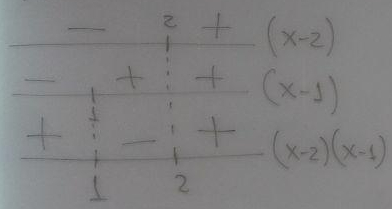
\includegraphics{\imgdirfromsection/[ok]photo_2018-08-24_22-55-35.jpg}
        \caption{}
    \end{figure}

    Assim, $S = \conjunto{ x \nos \reais \taisque x < 1 \ou x > 2 }$. Ademais, a solução $S\linha$ para a inequação $x^2 - 3x + 2 \menorigual 0$ pode ser obtida da seguinte forma:
    \begin{align*}
        S\linha &= S\complementar \\ 
                &= \conjunto{ x \nos \reais \taisque x < 1 \ou x > 2 }\complementar \\ 
                &= \conjunto{ x \nos \reais \taisque x \maiorigual 1 \e x \menorigual 2 } \\ 
                &= \conjunto{ x \nos \reais \taisque 1 \menorigual x \menorigual 2 }.
    \end{align*}
\end{solution}

\begin{example}
    Prove que a soma de um número positivo com seu inverso multiplicativo é sempre maior ou igual a 2.
\end{example}

\begin{proof}
    Queremos provar que $x+1/x\ge 2$, para todo $x > 0$. Note que:
    \begin{align*}
        x+\dfrac{1}{x}\ge 2 &\iff \dfrac{x^2+1-2x}{x}       \\
                            &\iff \dfrac{\prn{x-1}^2}{x}
    \end{align*}

    \begin{figure}[H]
        \centering
        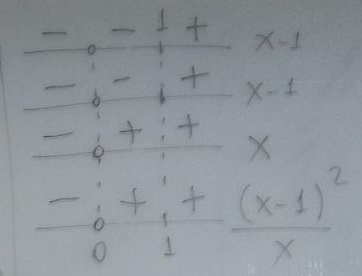
\includegraphics{\imgdirfromsection/[ok]photo_2018-08-24_22-55-35(2).jpg}
        \caption{}
    \end{figure}

    Logo, para que $x+1/x\ge 2$, é necessário e suficiente que $x > 0$, ou seja, $x$ é positivo.
\end{proof}